%!TEX program = xelatex
\documentclass[pdf]
{beamer}
\mode<presentation>{}

%% preamble
%\usetheme{metropolis}
\usepackage{blindtext}
\usetheme{Execushares}

\title{Análise de dados COVID-19 em Portugal}
\subtitle{Analysis of Portuguese COVID-19 data}
\author{João F. Pereira}
\date{7 Outubro 2022}

\setcounter{showSlideNumbers}{1}

\begin{document}
	
%%Title
\begin{frame}
\titlepage
\end{frame}

%%Content
\begin{frame}
	\frametitle{Índice}
	\begin{enumerate}
		\item Introdução
			\\ \textcolor{ExecusharesGrey}{\footnotesize\hspace{1em }Modelos Epidemiológicos}
		\item Como Realizar uma análise exploratória  \\ \textcolor{ExecusharesGrey}{\footnotesize\hspace{1em} Just some Lorem Ipsum for filler}
		\item Demonstração Prática \\ \textcolor{ExecusharesGrey}{\footnotesize\hspace{1em} Some closing thoughts}
		\item Conclusões
	\end{enumerate}
\end{frame}
	
	
%% Introdução
\begin{frame}{Introdução}
\begin{columns}
	\begin{column}[T]{0.65\textwidth}
		\vspace{1.5cm}
		\centering
		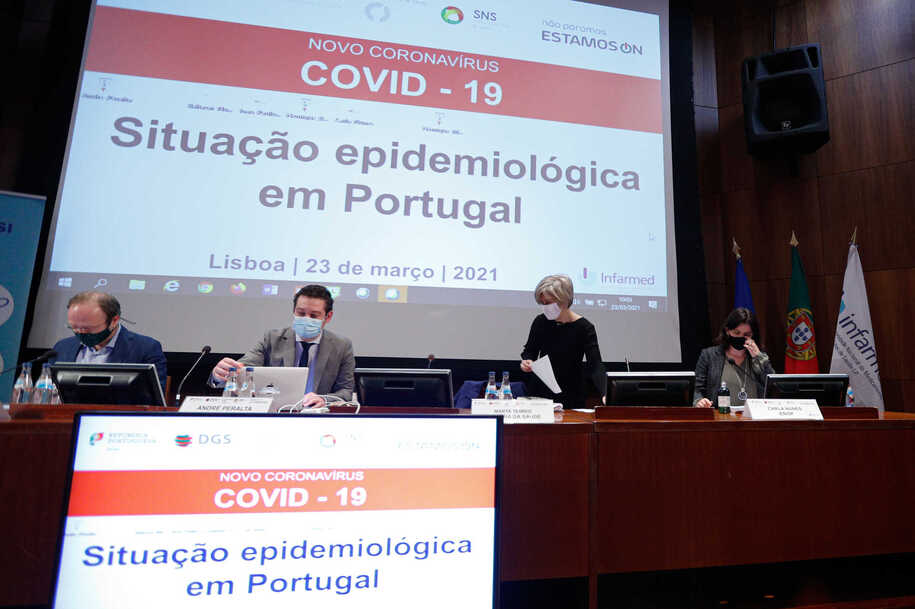
\includegraphics[width=\textwidth]{Imagens/Reunioes_Infarmed.jpg}\\
		\hfill \textcolor{ExecusharesGrey}{\tiny jn.pt, 23 Março 2021. Fonte: Lusa}
	\end{column}
	
	\begin{column}[T]{0.35\textwidth}
		\vspace{0.5cm}
		\textcolor {green}{\Large\textbf{COVID-19 inCTRL}}\\
		\textcolor{ExecusharesGrey}{\tiny\hspace{1em}Financiado pelo programa RESEARCH4COVID - FCT}
		\vspace{0.5cm}
		
\includegraphics[width=\textwidth]{Imagens/logo_utad_completo_azul.png}\\
		\vspace{0.3cm}
		
\includegraphics[width=\textwidth]{Imagens/logoentidade_INSA.png}\\
		%Bolsa Refª: COVID_inCTRL/DEP/01/2020\\
		%(de 11 Nov. 2020 até 10 Maio 2021)
	\end{column}
\end{columns}
\end{frame}

%% Modelos Epidemiológicos
\begin{frame}{Modelos Epidemiológicos}
\begin{columns}
	\begin{column}[T]{0.5\textwidth}
	\centering
		\vspace{0.2cm}
		\alert{\large Modelo SIR}\\
		\vspace{0.5cm}
		
\includegraphics[width=\textwidth]{Imagens/SIR_diagram.png}\\
		\vspace{-0.2cm}
		\begin{equation*}
		    \begin{cases}
			    \frac{dS}{dt} = -\beta \frac{S I}{N}\\
			    \frac{dI}{dt} = \frac{S I}{N} - \gamma I\\
			    \frac{dR}{dt} = \gamma I
		    \end{cases}
		\end{equation*}
		
		% Kermack-eta-A.-G.-McKendrick
		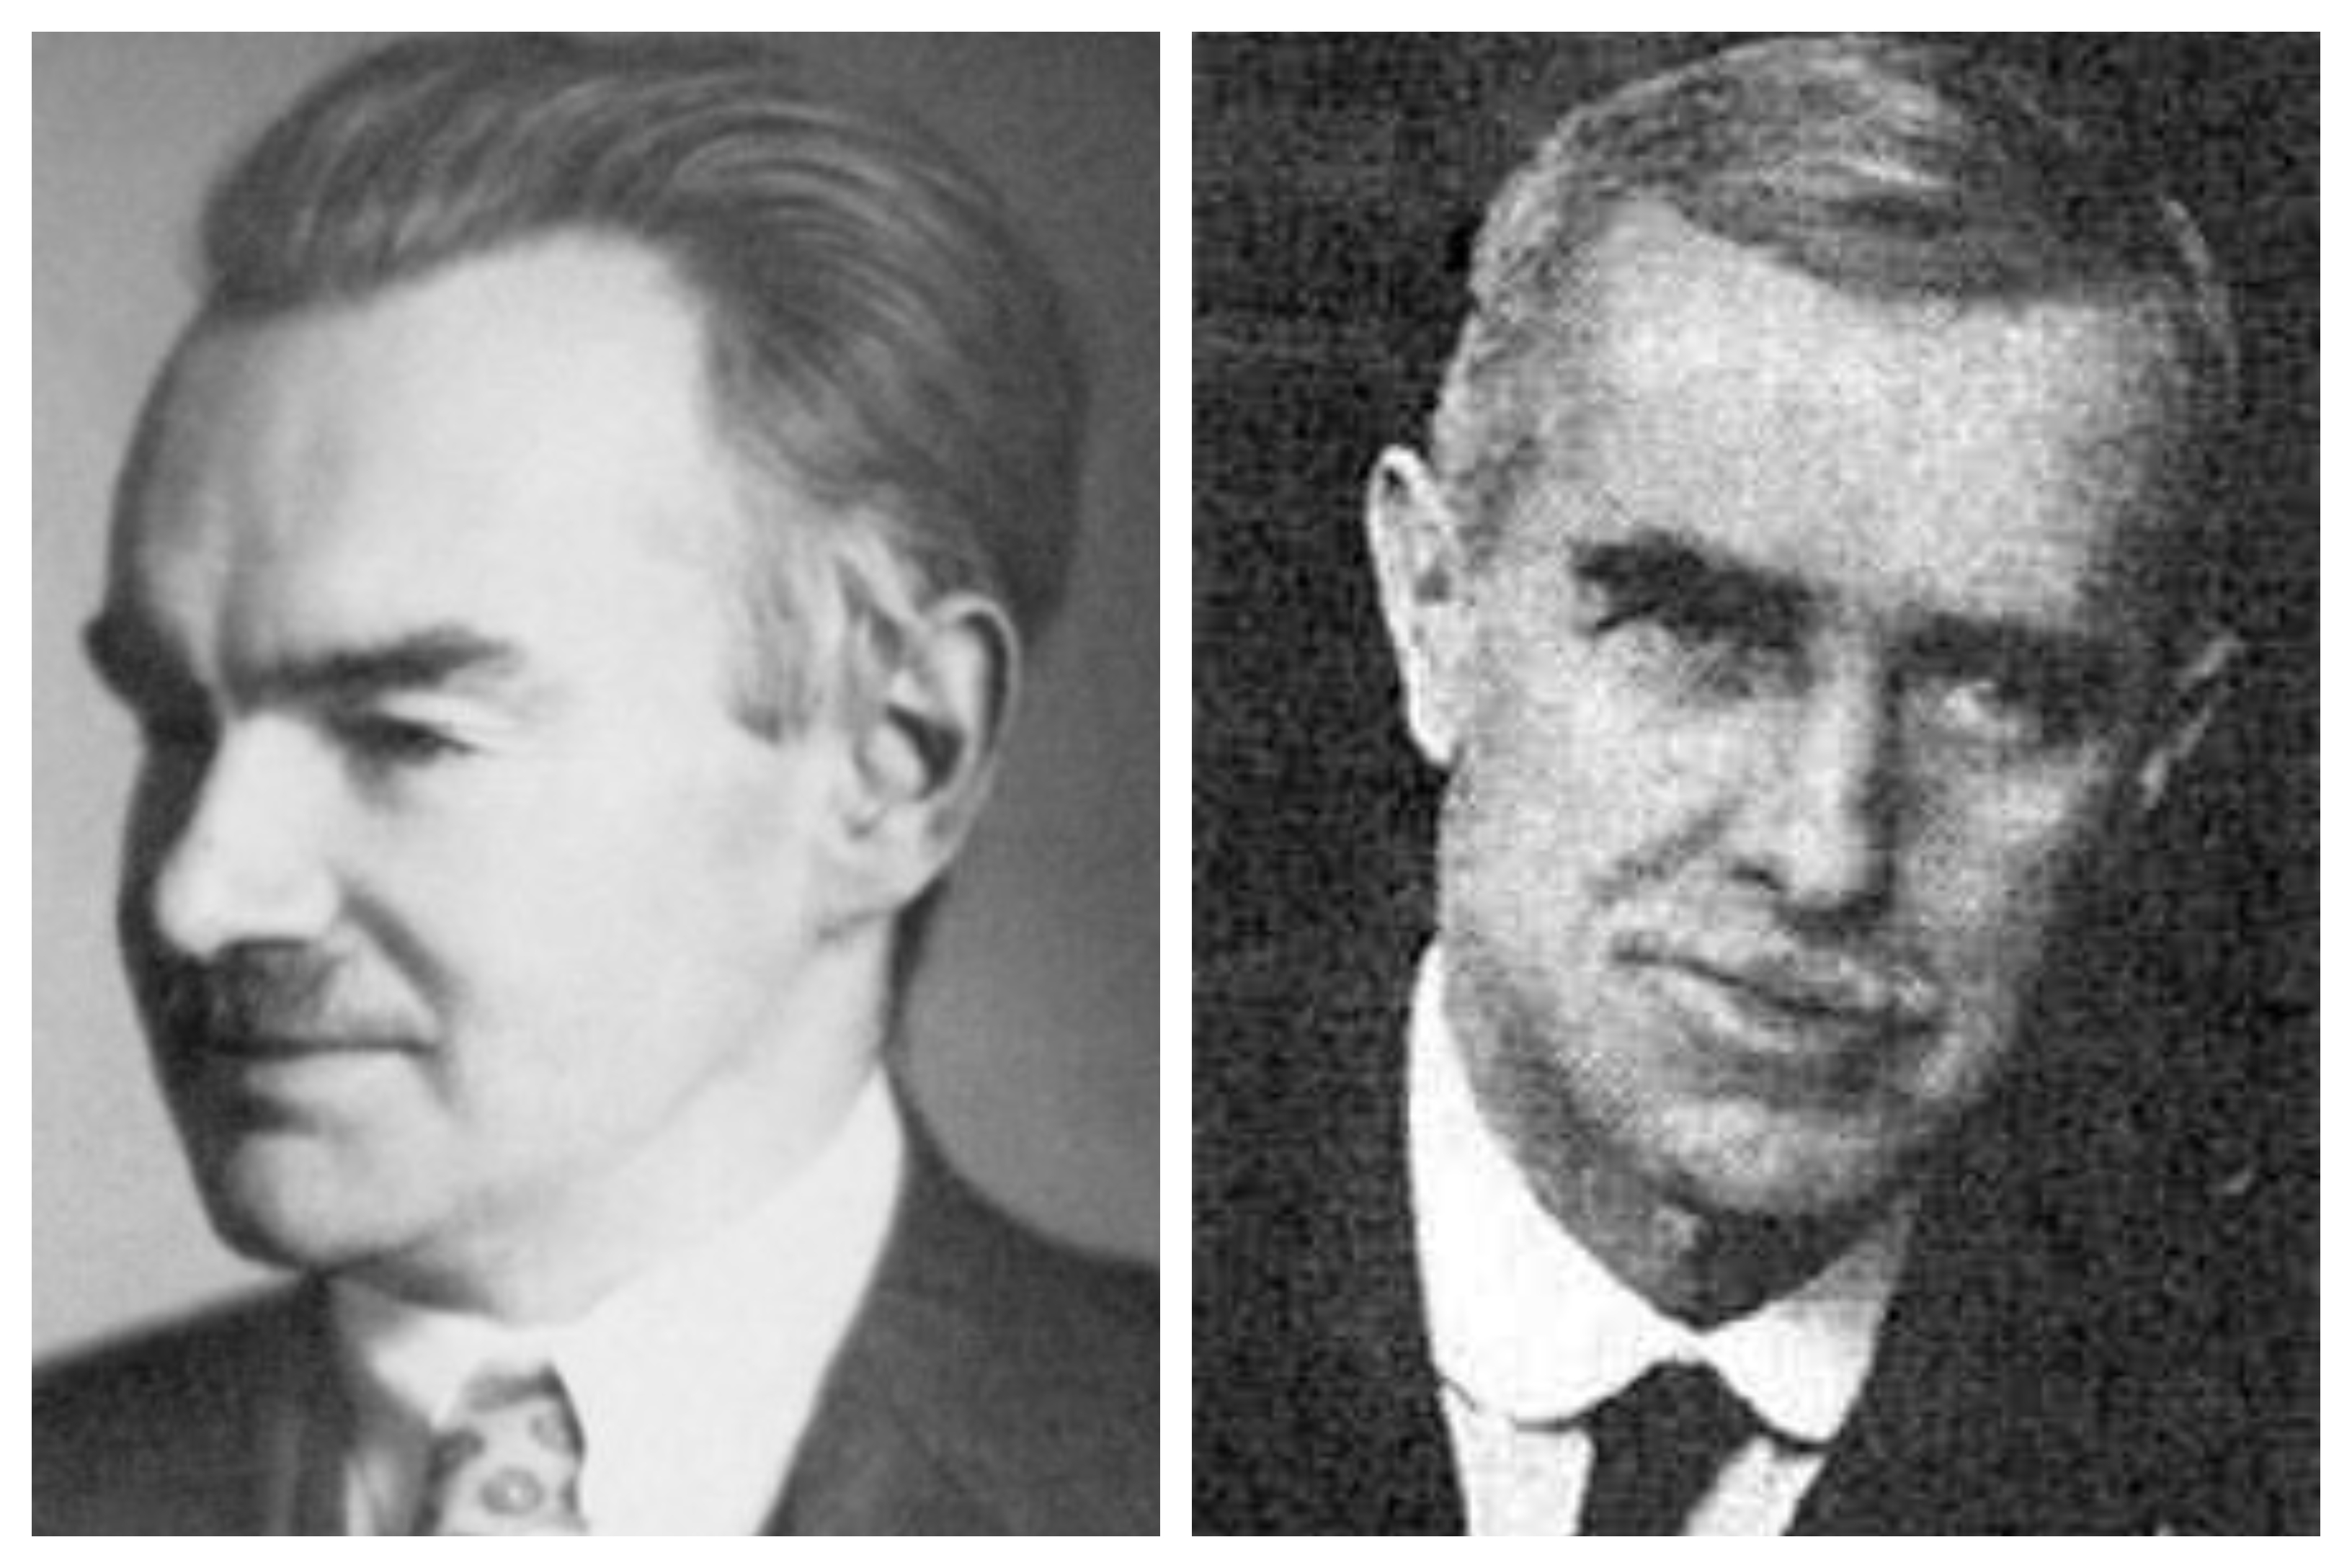
\includegraphics[width=0.5\textwidth]{Imagens/Kermack-eta-A.-G.-McKendrick.jpg}\\
		\textcolor{ExecusharesGrey}{\tiny W.O. Kermack e A.G. McKendrick}\\
	\end{column}
	
	\begin{column}[T]{0.5\textwidth}
		\centering
		\vspace{1.8cm}
		\alert{\large Modelo SEIR}\\
		\vspace{0.5cm}
		
\includegraphics[width=\textwidth]{Imagens/SEIR_diagram.png}\\
		\vspace{-0.2cm}
		\begin{equation*}
		    \begin{cases}
			    \frac{dS}{dt} = -\beta \frac{S I}{N}\\
			    \frac{dE}{dt} = \beta \frac{S I}{N} - \epsilon E\\
			    \frac{dI}{dt} = \epsilon E - \gamma I\\
			    \frac{dR}{dt} = \gamma I
		    \end{cases}
		\end{equation*}
		
	\end{column}
\end{columns}
\end{frame}

%%
\begin{frame}{Modelos Epidemiológicos}
\begin{columns}
	\begin{column}[T]{0.6\textwidth}
		\centering
		\vspace{0.6cm}
		\alert{\large Modelo COVID-19 inCTRL}\\
		\vspace{0.5cm}
		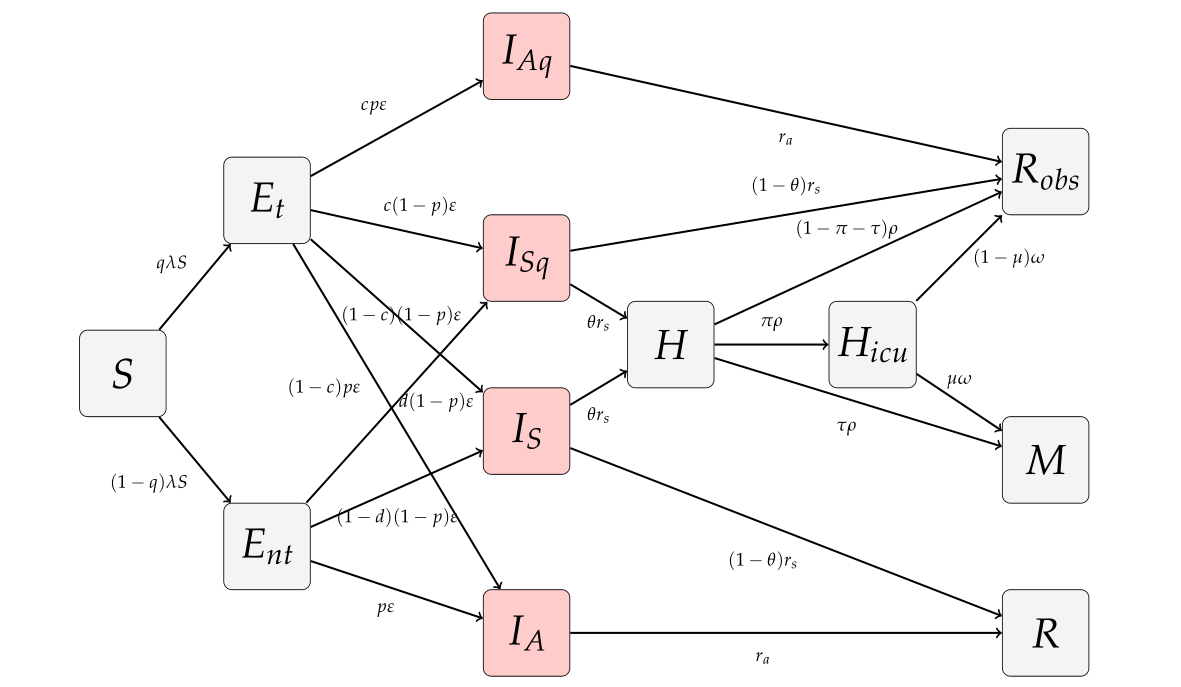
\includegraphics[width=0.8\textwidth]{Imagens/InCTRL_model.png}\\
		\vspace{0.5cm}
		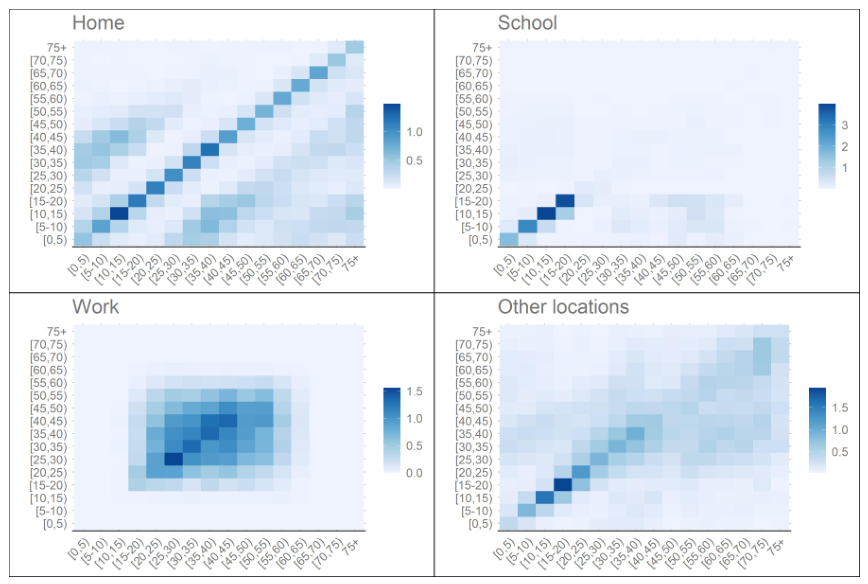
\includegraphics[width=0.7\textwidth]{Imagens/Cont_Matrix.png}\\
	\end{column}
	
	\begin{column}[T]{0.4\textwidth}
		\tiny
		\begin{equation*}
		        \begin{aligned}
		            S' &= -\lambda S,\\
		            E'_t &= q \lambda S - \epsilon E_t\\
		            I'_A &= p \epsilon E_{nt} + (1-c)p \epsilon E_t - r_a I_A\\
		            I'_S &= (1-d)(1-p) \epsilon E_{nt} + (1-c)(1-p) \epsilon E_t - r_s I_S\\
		            E'_{nt} &= (1-q) \lambda S - \epsilon E_{nt}\\
		            I'_{Aq} &= c p \epsilon E_t - r_a I_{Aq}\\
		            I'_{Sq} &= c(1-p) \epsilon E_t + d (1-p) \epsilon E_{nt} - r_s I_{Sq}\\
		            H' &= \theta r_s (I_S + I_{Sq}) - \rho H\\
		            H'_{icu} &= \pi \rho H - \omega H_{icu}\\
		            M' &= \mu \omega H_{icu} + \tau \rho H\\
		            R'_{obs} &= (1-\theta) r_s I_{Sq} + r_a I_{Aq} + (1-\pi-\tau)\rho H + (1-\mu)\omega H_{icu}\\
		            R' &= (1-\theta) r_s I_S + r_a I_A
		        \end{aligned}
		\end{equation*}
		%\vspace{0.5cm}
		\vfill
		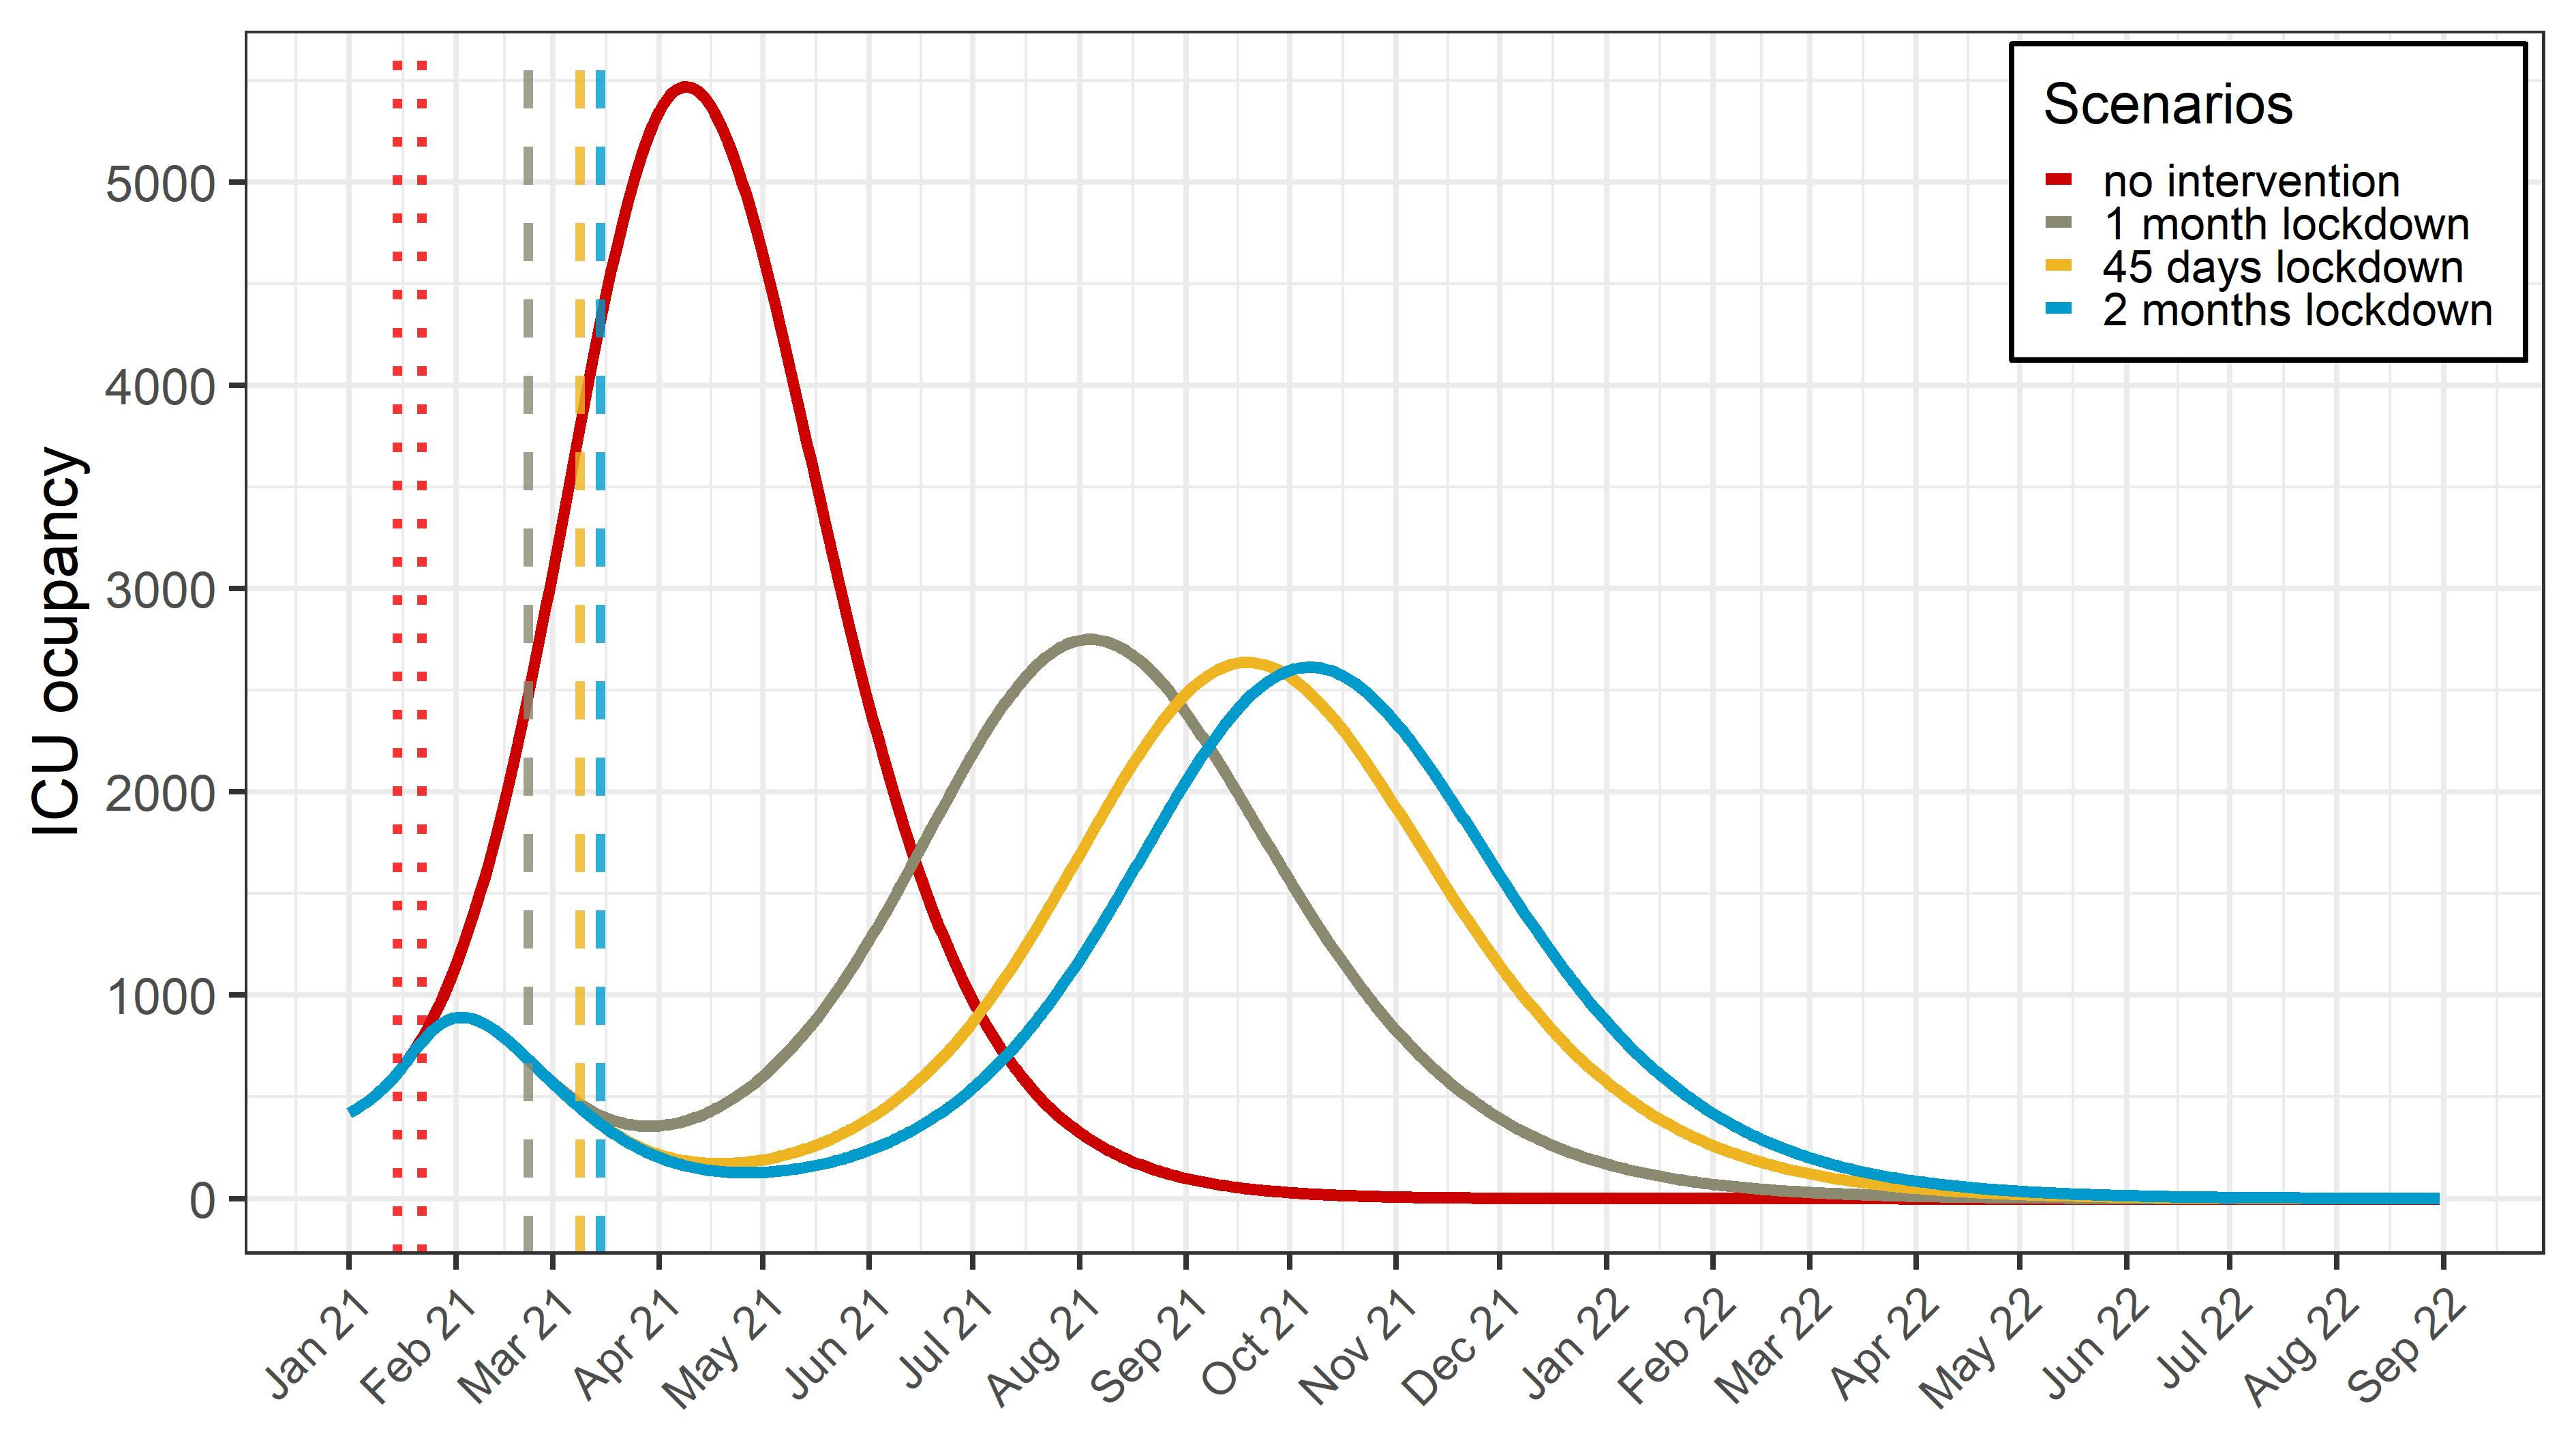
\includegraphics[width=\textwidth]{Imagens/inCTRL_Scenarios_ICU.jpg}\\
	\end{column}
\end{columns}
\end{frame}

	
\end{document}

